\documentclass{beamer}

\usetheme{Madrid}

\usepackage[utf8]{inputenc}
\usepackage[T1]{fontenc}
\usepackage{graphicx}
\usepackage{booktabs}
\usepackage{amsmath}

\title{Project 2: YSU Quantitative Finance}
\author{Aramayis, Armen, Tigran}
\institute{Yerevan State University}
\date{June - 17, 2026}

\begin{document}

\frame{\titlepage}

\begin{frame}{Outline}
    \tableofcontents
\end{frame}





\section{Project 2b - Bayesian Update}

\begin{frame}{Bayesian Updates: Bernoulli Data}
    Model each binary outcome $X_i \in \{0,1\}$ (e.g. is the daily return positive?) as
    $X_i \overset{iid}{\sim} \text{Bernoulli}(p)$.

    \textbf{Prior:} $p \sim \text{Beta}(a, b)$, default $a = b = 1$ (Uniform)

    \textbf{Posterior} (conjugacy), with $s = \sum x_i$ successes out of $n$:
    \[
        p \mid \text{data} \sim \text{Beta}(a+s,\ b+n-s)
    \]

    \textbf{Estimates} from posterior $\text{Beta}(a', b')$:
    \[
        \hat{p}_{\text{MAP}} = \frac{a'-1}{a'+b'-2}, \qquad
        \hat{p}_{\text{Bayes}} = \frac{a'}{a'+b'}
    \]
    \begin{itemize}
        \item \textbf{Why Beta?} Beta is the conjugate prior for Bernoulli because the posterior
              has the same Beta functional form as the prior -- updating reduces to incrementing
              the shape parameters: $a' = a + s$,\ $b' = b + (n-s)$
    \end{itemize}
\end{frame}

\begin{frame}{Bernoulli Example: Toy Data}
    Prior $\text{Beta}(1,1)$, data \texttt{1100101100} ($n=10$, $s=5$ successes)
    \begin{center}
        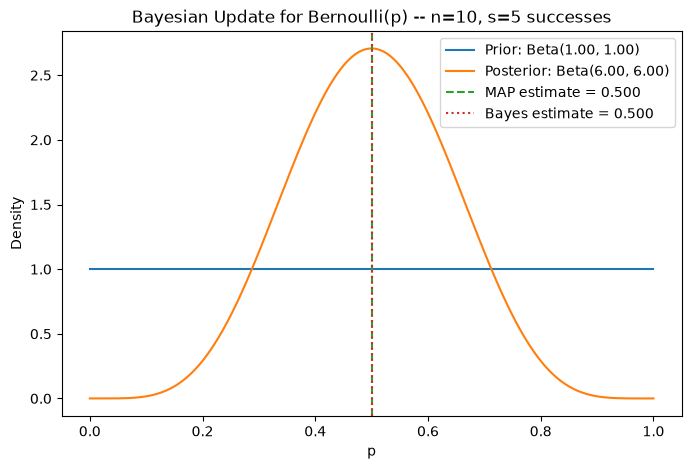
\includegraphics[width=0.6\textwidth]{../figures/bernoulli_dashboard.png}
    \end{center}
    Posterior $\text{Beta}(6,6)$, \quad $\hat{p}_{\text{MAP}} = \hat{p}_{\text{Bayes}} = 0.500$
    \begin{itemize}
        \item MAP and Bayes estimates coincide here because $\text{Beta}(6,6)$ is symmetric;
              for an asymmetric posterior they would generally differ
    \end{itemize}
\end{frame}

\begin{frame}{Bernoulli Example: Is AAPL's Daily Return Positive?}
    $X_t = 1$ if AAPL's daily log return is positive, $0$ otherwise. Prior $\text{Beta}(1,1)$,
    $n = 1356$ days, $s = 719$ positive days.
    \begin{center}
        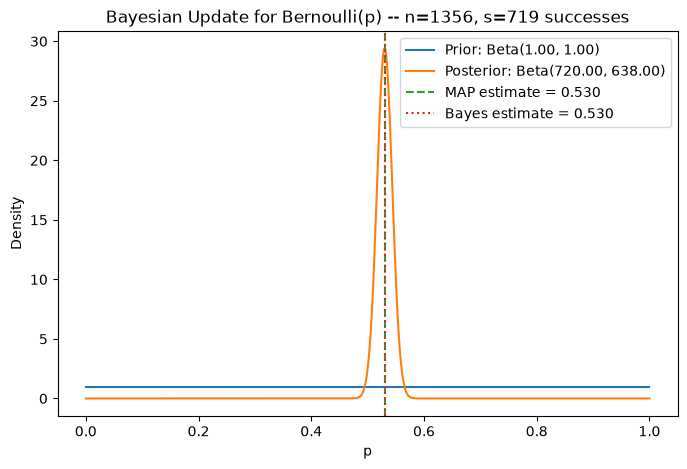
\includegraphics[width=0.6\textwidth]{../figures/bernoulli_aapl.png}
    \end{center}
    Posterior $\text{Beta}(720, 638)$, \quad $\hat{p}_{\text{MAP}} = \hat{p}_{\text{Bayes}} \approx 0.530$
    \begin{itemize}
        \item AAPL closes up on $\approx 53\%$ of days -- slightly more often than not
        \item 95\% credible interval: $[0.5036,\ 0.5567]$ -- AAPL closes up slightly more
              than half the time, but with meaningful uncertainty remaining
    \end{itemize}
\end{frame}

\begin{frame}{Bayesian Updates: Normal Data}
    Model $X_i \overset{iid}{\sim} N(\mu, \sigma^2)$ with \textbf{known} $\sigma$ (e.g. the
    mean daily return $\mu$ of a stock).

    \textbf{Prior:} $\mu \sim N(\mu_0, \sigma_0^2)$, default $\mu_0 = 0$, $\sigma_0 = 1$

    \textbf{Posterior} (conjugacy), with sample mean $\bar{x}$:
    \[
        \mu \mid \text{data} \sim N(\mu_n, \sigma_n^2), \qquad
        \frac{1}{\sigma_n^2} = \frac{1}{\sigma_0^2} + \frac{n}{\sigma^2}, \qquad
        \mu_n = \sigma_n^2\left(\frac{\mu_0}{\sigma_0^2} + \frac{n\bar{x}}{\sigma^2}\right)
    \]

    For a Normal posterior, mode = mean:
    \[
        \hat{\mu}_{\text{MAP}} = \hat{\mu}_{\text{Bayes}} = \mu_n
    \]
\end{frame}

\begin{frame}{Normal Example: Toy Data}
    $\sigma = 1$, prior $N(0,1)$, data $0.123,\ 1.3812,\ -0.13$ ($n=3$)
    \begin{center}
        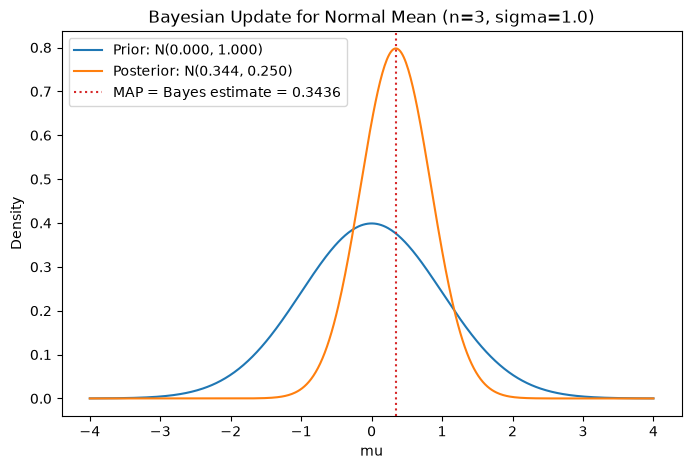
\includegraphics[width=0.6\textwidth]{../figures/normal_dashboard.png}
    \end{center}
    Posterior $N(0.344,\ 0.25)$, \quad $\hat{\mu}_{\text{MAP}} = \hat{\mu}_{\text{Bayes}} = 0.344$
\end{frame}

\begin{frame}{Normal Example: Mean of AAPL Daily Returns}
    $\sigma$ fixed at the sample std of AAPL's log returns, prior $N(0,1)$, $n = 1356$
    \begin{center}
        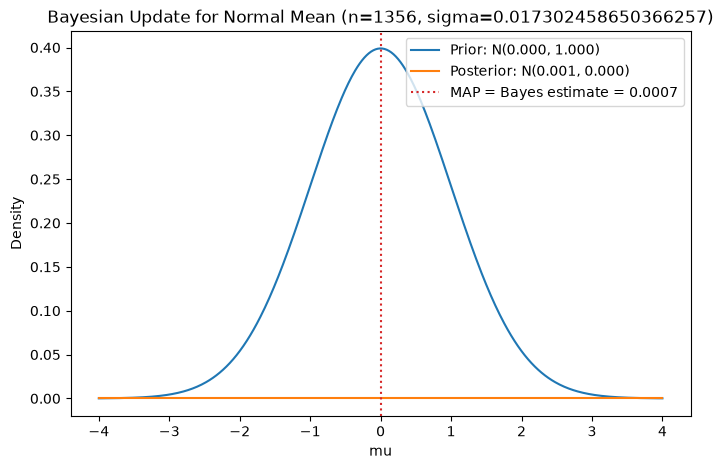
\includegraphics[width=0.6\textwidth]{../figures/normal_aapl.png}
    \end{center}
    Posterior mean $\hat{\mu}_{\text{Bayes}} \approx 0.0007$ -- with $n = 1356$, the data
    completely dominates the (wide) prior
    \begin{itemize}
        \item $0.07\%$ daily return compounds to approximately $19.28\%$ annually
              (252 trading days) -- statistically detectable but economically modest drift
    \end{itemize}
\end{frame}

\begin{frame}{Why Bayes? From Estimate to Decision}
    A frequentist gives a point estimate $\hat{p} = 0.530$ and a confidence interval.

    The Bayesian posterior gives the \textbf{full probability distribution} over $p$ --
    so we can make direct probability statements:
    \begin{itemize}
        \item $P(p > 0.5 \mid \text{data}) = 0.987$ \quad ($98.7\%$)
        \item $P(p < 0.5 \mid \text{data}) = 0.013$ \quad ($1.3\%$)
    \end{itemize}
    We are $\mathbf{98.7\%}$ confident AAPL is an upward-drifting asset -- a statement
    a frequentist confidence interval cannot make directly.
\end{frame}

\begin{frame}{Supplementary: Does the Posterior Forget the Prior?}
    Known true $\mu = 2$, $\sigma = 1$; prior $N(0,1)$ (deliberately off-center). Generate
    $n$ points from the true distribution and compute the posterior.
    \begin{center}
        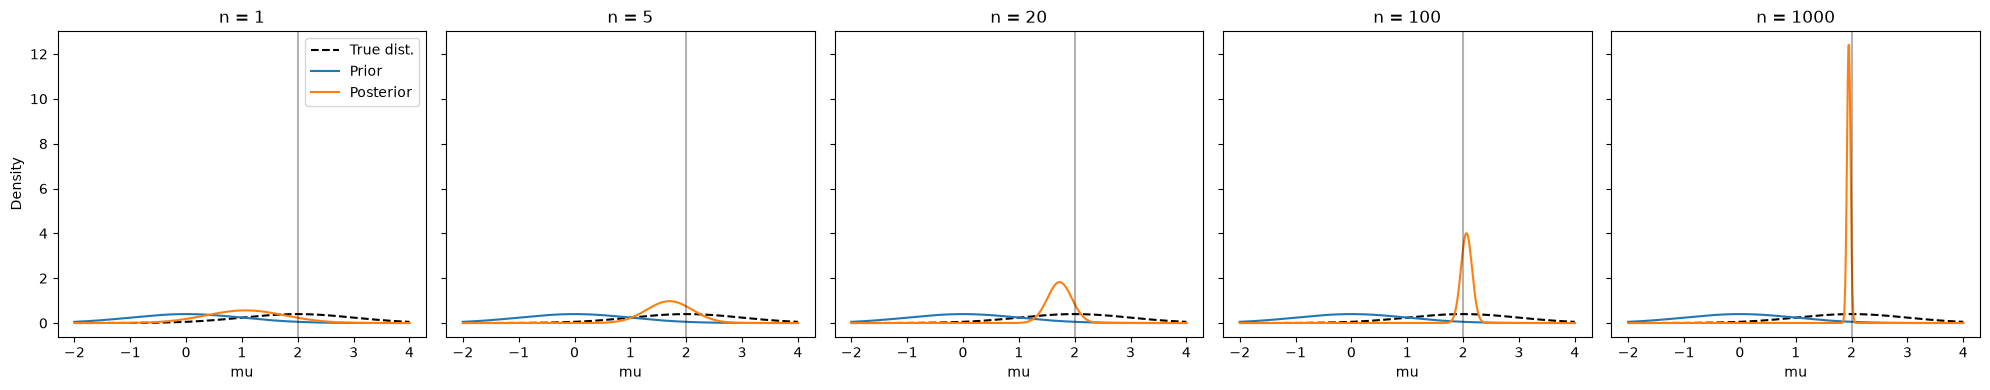
\includegraphics[width=0.95\textwidth]{../figures/normal_convergence.png}
    \end{center}
    \begin{itemize}
        \item As $n$ grows, the posterior narrows and shifts toward the true $\mu$
        \item The prior's influence vanishes as $n \to \infty$
        \item \textbf{Bernstein--von Mises theorem:} as $n \to \infty$, the posterior
              converges to a Normal distribution centered at the true parameter, with
              variance equal to the inverse Fisher information -- regardless of the prior
        \item \textbf{Implication:} with enough data, Bayesian and frequentist inference
              agree. The prior only matters when data is scarce
    \end{itemize}
\end{frame}



















\begin{frame}{What the Three Methods Agree On}
    \begin{itemize}
        \item \textbf{Linear Regression:} only contemporaneous information explains
              returns -- lagged predictors have $R^2 \approx 0$
        \item \textbf{Bayesian Analysis:} stable long-run parameters exist
              ($\hat{p} \approx 0.530$,\ $\hat{\mu} \approx 0.0007$) but with
              uncertainty quantified via the full posterior
        \item \textbf{Markov Chains:} regime structure is persistent, but mechanically
              so due to the rolling-window construction
        \item \textbf{Common thread:} weak-form market efficiency -- daily prices are
              unpredictable, but statistical structure exists at longer timescales
    \end{itemize}
\end{frame}

\section{Project 2c - Linear Regression Models}

% ===================== DATA & METHODOLOGY =====================
\begin{frame}{Data and Methodology}
    \begin{itemize}
        \item \textbf{Selection:} stocks from one sector --- \textbf{Technology} (5 names):
              \texttt{AAPL}, \texttt{MSFT}, \texttt{NVDA}, \texttt{GOOGL}, \texttt{META}
        \item \textbf{Market index:} \texttt{\^{}GSPC} (S\&P 500)
        \item \textbf{Period:} 2021-01-01 to 2026-06-01, daily ($\approx 1356$ obs)
        \item \textbf{Variable:} daily log returns $r_t = \log\!\left(P_t/P_{t-1}\right)$
        \item \textbf{Method:} OLS via \texttt{statsmodels}; inference re-run with
              heteroskedasticity / autocorrelation-robust (HC/HAC) standard errors
    \end{itemize}
\end{frame}

\begin{frame}{Strong Co-movement Across the Sector}
    Daily-return correlations among the five tech stocks and the index.
    \begin{center}
        
\includegraphics[width=0.55\textwidth]{Screenshot 2026-06-26 at 12.24.21.png}
    \end{center}
    \begin{itemize}
        \item All pairs are strongly positively correlated -- the stocks move together
        \item This is the ``can one stock explain another?'' question: the answer is
              \emph{yes}, but it reflects a \textbf{shared market factor}, not a direct link
    \end{itemize}
\end{frame}

% ===================== STAGE 1 =====================
\begin{frame}{Stage 1: Three Simple Linear Regressions}
    For each stock we fit three single-predictor models (shown here for \texttt{AAPL}):
    \begin{align*}
        \text{(A) Market:}        && \text{AAPL}_t &= \beta_0 + \beta_1\,\text{S\&P 500}_t + \varepsilon_t\\[2pt]
        \text{(B) Lagged market:} && \text{AAPL}_t &= \beta_0 + \beta_1\,\text{S\&P 500}_{t-1} + \varepsilon_t\\[2pt]
        \text{(C) Own lag (AR1):} && \text{AAPL}_t &= \beta_0 + \beta_1\,\text{AAPL}_{t-1} + \varepsilon_t
    \end{align*}
    \begin{itemize}
        \item (A) Can the market index explain individual stock returns?
        \item (B), (C) Can past returns predict future returns?
    \end{itemize}
\end{frame}

\begin{frame}{Model A: Market Model (contemporaneous)}
    \textbf{Can market index returns explain individual stock returns?}
    \[
        \text{Stock}_t = \beta_0 + \beta_1 \cdot \text{S\&P 500}_t + \varepsilon_t
    \]
    \begin{center}
        
\includegraphics[width=0.92\textwidth]{Unknown-6.png}
    \end{center}
    Each panel: stock return vs same-day S\&P 500 return ($\beta$, $R^2$ in titles).
\end{frame}

\begin{frame}{Model A: Results}
    \begin{table}
        \centering\footnotesize
        \begin{tabular}{lccccc}
            \toprule
            & AAPL & MSFT & NVDA & GOOGL & META \\
            \midrule
            $\beta$ (market) & $1.229$ & $1.140$ & $2.146$ & $1.272$ & $1.599$ \\
            $R^2$            & $0.556$ & $0.526$ & $0.491$ & $0.468$ & $0.385$ \\
            \bottomrule
        \end{tabular}
    \end{table}
    \begin{itemize}
        \item All five betas are large and \textbf{highly significant} ($p \approx 0$);
              $\beta$ is the stock's \textbf{market beta} (systematic-risk loading)
        \item Every $\beta > 1$ (NVDA highest at $2.15$, MSFT lowest at $1.14$) --
              these tech names amplify market moves
        \item $R^2 \approx 0.39$--$0.56$: the market explains a large share of each
              stock's daily variance; the rest ($1-R^2$) is idiosyncratic
        \item Intercept $\alpha$ (Jensen's alpha) is \textbf{not} significant --
              no abnormal return once market risk is accounted for
        \item Residuals are fat-tailed (heavy tails in the Q--Q plot) -- typical of daily returns
    \end{itemize}
\end{frame}

\begin{frame}{Model B: Lagged Market $\to$ Stock Return}
    \textbf{Can yesterday's market move predict today's return?}
    \[
        \text{Stock}_t = \beta_0 + \beta_1 \cdot \text{S\&P 500}_{t-1} + \varepsilon_t
    \]
    \begin{center}
        
\includegraphics[width=0.92\textwidth]{Unknown-7.png}
    \end{center}
    \begin{itemize}
        \item Slopes $\approx 0$, \textbf{not significant}, $R^2 \approx 0$ for every stock
        \item Lagged index return has \textbf{no} predictive power -- weak-form efficiency
    \end{itemize}
\end{frame}

\begin{frame}{Model C: Own Lagged Return (AR1)}
    \textbf{Does a stock's own past return predict its next return?}
    \[
        \text{Stock}_t = \beta_0 + \beta_1 \cdot \text{Stock}_{t-1} + \varepsilon_t
    \]
    \begin{center}
        
\includegraphics[width=0.92\textwidth]{Unknown-8.png}
    \end{center}
    \begin{itemize}
        \item Daily autocorrelation is tiny ($\beta_1 \approx 0$), $R^2 \approx 0$
        \item Returns behave like white noise -- no momentum / mean-reversion to exploit
    \end{itemize}
\end{frame}

\begin{frame}{Stage 1: Summary}
    \begin{table}
        \centering
        \begin{tabular}{lccc}
            \toprule
            Model & Predictor & $R^2$ & Significant? \\
            \midrule
            A & S\&P 500$_t$     & $0.556$ & Yes \\
            B & S\&P 500$_{t-1}$ & $\approx 0.000$ & No \\
            C & AAPL$_{t-1}$     & $\approx 0.000$ & No \\
            \bottomrule
        \end{tabular}
        \\[2pt]
        {\footnotesize (R$^2$ shown for AAPL; full sector range in Model A is $0.39$--$0.56$.)}
    \end{table}
    \begin{itemize}
        \item Same-day market index return strongly explains each stock's return
              ($R^2 \approx 0.39$--$0.56$ across the sector)
        \item Lagged (past) returns -- index or own -- carry \textbf{no} predictive
              information: consistent with weak-form market efficiency
        \item Cross-stock co-movement (e.g. GOOGL vs AAPL) is really shared exposure to
              this same market factor
    \end{itemize}
\end{frame}

% ===================== STAGE 2 =====================
\begin{frame}{Stage 2: Multiple Linear Regression}
    Predict a target stock's return from \textbf{several predictors jointly}:
    \footnotesize
    \[
        \text{AAPL}_t = \beta_0 + \beta_1 \text{S\&P 500}_t + \beta_2 \text{S\&P 500}_{t-1}
        + \beta_3 \text{AAPL}_{t-1} + \beta_4 \text{AAPL}_{t-2}
    \]
    \[
        \qquad\quad + \beta_5 \text{MAgap}_{t-1} + \beta_6 \text{Vol}_{t-1}
        + \beta_7 \text{RelVol}_{t-1} + \varepsilon_t
    \]
    \normalsize
    \begin{itemize}
        \item \texttt{MAgap}: price vs its 20-day moving average; \texttt{Vol}: 20-day
              realised volatility; \texttt{RelVol}: volume vs its 20-day average
        \item All predictors except the same-day market are \textbf{strictly lagged} --
              no look-ahead, so a model without S\&P 500$_t$ is genuinely usable to forecast
    \end{itemize}
\end{frame}

\begin{frame}{Stage 2: Results (AAPL full model)}
    \begin{center}
        
\includegraphics[width=0.95\textwidth]{Unknown-9.png}
    \end{center}
    \begin{itemize}
        \item Only the \textbf{same-day market} term is significant; its coefficient
              matches the Stage-1 beta
        \item $R^2 \approx 0.57$, adjusted $R^2 \approx 0.56$ -- barely above the
              market-only model; lagged \& technical predictors add almost nothing
        \item All VIFs $< 5$ -- no multicollinearity; the predictors simply carry no signal
        \item Residuals-vs-fitted fans out -- volatility clustering (heteroskedasticity)
    \end{itemize}
\end{frame}

% ===================== STAGE 3 =====================
\begin{frame}{Stage 3: Model Selection (in- vs out-of-sample)}
    Candidate models fit on the \textbf{same sample}; out-of-sample uses a chronological
    80/20 split, benchmarked against the historical-mean forecast.
    \begin{center}
        
\includegraphics[width=0.7\textwidth]{Unknown-10.png}
    \end{center}
    \begin{itemize}
        \item AIC/BIC and adjusted $R^2$ prefer the parsimonious \textbf{market-only} model
        \item Market-inclusive models keep $R^2_{\text{OOS}} \approx 0.29$ -- but only because they
              use the \emph{same-day} market return (not a true forecast)
        \item The honest lagged-only model has $R^2_{\text{OOS}} \approx 0$ (slightly negative):
              \textbf{past information cannot beat predicting the mean}
    \end{itemize}
\end{frame}

\begin{frame}{Stage 3: Residual Diagnostics}
    \begin{center}
        
\includegraphics[width=0.5\textwidth]{Unknown-11.png}
    \end{center}
    \begin{itemize}
        \item \textbf{Jarque--Bera} rejects normality -- heavy tails, visible in the Q--Q tails
        \item \textbf{Breusch--Pagan} rejects homoskedasticity -- variance clusters (scale--location fans out)
        \item \textbf{Durbin--Watson} $\approx 2$ and Ljung--Box insignificant -- no exploitable autocorrelation
        \item $\Rightarrow$ point estimates fine, but we report \textbf{HC/HAC robust} standard errors
    \end{itemize}
\end{frame}

% ===================== STAGE 4 (EXTENSION) =====================
\begin{frame}{Extension: Beta Is Not Constant}
    Re-estimate the market model on a rolling 120-day window: $\hat\beta_t$ over time.
    \begin{center}
        
\includegraphics[width=0.95\textwidth]{Unknown-14.png}
    \end{center}
    \begin{itemize}
        \item The single Stage-1 beta is a 5-year \emph{average} -- the true loading drifts a lot
        \item Betas climb inside market drawdowns (shaded): in selloffs correlations
              spike and \textbf{everything moves together} -- risk is state-dependent
    \end{itemize}
\end{frame}

\begin{frame}{Extension: Systematic Share Over Time}
    Rolling $R^2$ of the market model -- the fraction of variance the market explains.
    \begin{center}
        
\includegraphics[width=0.92\textwidth]{Unknown-13.png}
    \end{center}
    \begin{itemize}
        \item $R^2$ rises in stressed periods -- the market dominates exactly when
              diversification is least helpful
    \end{itemize}
\end{frame}

\begin{frame}{Linear Regression: Summary}
    \begin{itemize}
        \item \textbf{Market explains, contemporaneously:} same-day index return is the
              dominant driver ($R^2 \approx 0.39$--$0.56$); its slope is the stock's beta
        \item \textbf{Past returns do not predict:} lagged index, own lags, moving-average,
              volatility and volume are jointly insignificant and fail out-of-sample
        \item \textbf{Volume:} does not explain the \emph{signed} daily return
        \item \textbf{Best model} = the market model; \textbf{best genuine predictor} = the mean
        \item \textbf{Beta is dynamic:} it rises in drawdowns -- a static regression hides
              the risk exactly when it matters most
        \item Overall: consistent with \textbf{weak-form efficiency with time-varying volatility}
              -- the conditional \emph{mean} is unpredictable, the \emph{variance} is not
    \end{itemize}
\end{frame}

\section{Project 2c - Markov Chain Models}

\begin{frame}{Defining Market Regimes}
    Classify each day's NASDAQ Composite (\texttt{\^{}IXIC}) into \textbf{Bull}, \textbf{Neutral},
    or \textbf{Bear} using the 20-day rolling cumulative log return
    \[
        R_t = \sum_{i=0}^{19} r_{t-i}, \qquad \theta = 0.5 \cdot \text{std}(R_t)
    \]
    \[
        \text{Regime}_t =
        \begin{cases}
            \text{Bull}    & R_t > \theta \\
            \text{Bear}    & R_t < -\theta \\
            \text{Neutral} & \text{otherwise}
        \end{cases}
    \]
    \begin{table}
        \centering
        \begin{tabular}{lccc}
            \toprule
            Regime & Bull & Neutral & Bear \\
            \midrule
            Days (\%) & $554$ ($41.4\%$) & $465$ ($34.8\%$) & $318$ ($23.8\%$) \\
            \bottomrule
        \end{tabular}
    \end{table}
\end{frame}

\begin{frame}{NASDAQ Composite Colored by Regime}
    \begin{center}
        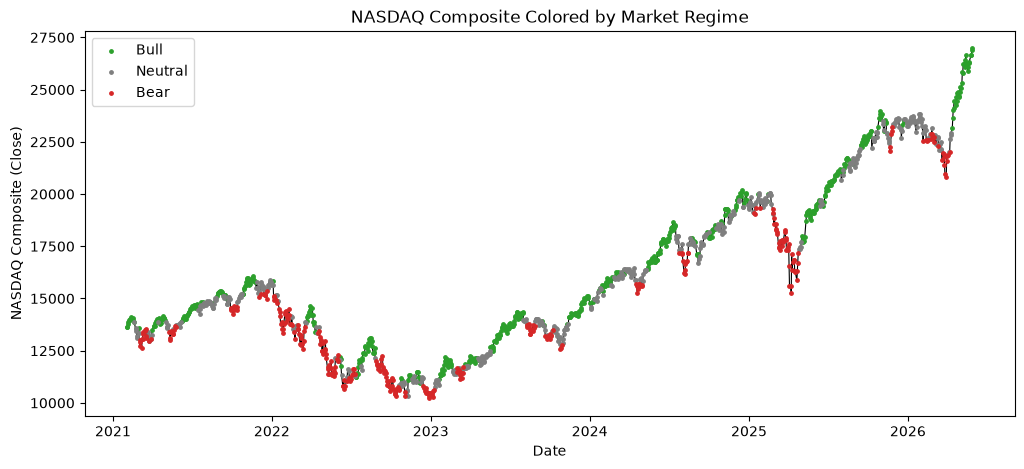
\includegraphics[width=0.95\textwidth]{../figures/regime_plot.png}
    \end{center}
\end{frame}

\begin{frame}{Transition Probability Matrix}
    \[
        P_{ij} = P(\text{Regime}_{t+1} = j \mid \text{Regime}_t = i)
    \]
    \[
        P =
        \begin{pmatrix}
            0.879 & 0.121 & 0.000 \\
            0.144 & 0.751 & 0.105 \\
            0.000 & 0.154 & 0.846
        \end{pmatrix}
        \quad \text{(rows/cols: Bull, Neutral, Bear)}
    \]
    \begin{itemize}
        \item All three regimes are highly \textbf{persistent} (diagonal $\approx 0.75$--$0.88$)
        \item $P(\text{Bull}\to\text{Bear}) = P(\text{Bear}\to\text{Bull}) = 0$ -- the market
              always passes through Neutral
    \end{itemize}
\end{frame}

\begin{frame}{Stationary Distribution}
    $\pi P = \pi$, $\sum_i \pi_i = 1$
    \begin{table}
        \centering
        \begin{tabular}{lcc}
            \toprule
            Regime & Stationary $\pi$ & Observed frequency \\
            \midrule
            Bull    & $0.414$ & $0.414$ \\
            Neutral & $0.348$ & $0.348$ \\
            Bear    & $0.238$ & $0.238$ \\
            \bottomrule
        \end{tabular}
    \end{table}
    \begin{itemize}
        \item Stationary distribution matches observed frequencies almost exactly --
              the chain is essentially already at its long-run distribution
    \end{itemize}
\end{frame}

\begin{frame}{Predicting the Next Regime}
    Given the current regime $i$, the most probable next regime is $\arg\max_j P_{ij}$.
    \begin{itemize}
        \item Last observed regime: \textbf{Bull}
        \item $P(\text{Bull} \to \text{Bull}) = 0.879$, \quad
              $P(\text{Bull} \to \text{Neutral}) = 0.121$, \quad
              $P(\text{Bull} \to \text{Bear}) = 0.000$
        \item \textbf{Predicted next regime: Bull}
    \end{itemize}
\end{frame}

\begin{frame}{Simulating the Markov Chain}
    Simulate a regime sequence of the same length from $P$ and compare to the observed data.
    \begin{table}
        \centering
        \begin{tabular}{lcc}
            \toprule
            & \multicolumn{2}{c}{Frequency} \\
            Regime & Observed & Simulated \\
            \midrule
            Bull    & $0.414$ & $0.476$ \\
            Neutral & $0.348$ & $0.301$ \\
            Bear    & $0.238$ & $0.223$ \\
            \bottomrule
        \end{tabular}
        \qquad
        \begin{tabular}{lcc}
            \toprule
            & \multicolumn{2}{c}{Avg. run length (days)} \\
            Regime & Observed & Simulated \\
            \midrule
            Bull    & $8.1$ & $8.8$ \\
            Neutral & $4.0$ & $3.3$ \\
            Bear    & $6.5$ & $6.0$ \\
            \bottomrule
        \end{tabular}
    \end{table}
    \begin{itemize}
        \item A first-order Markov chain reproduces both the regime frequencies and the
              average regime durations reasonably well
    \end{itemize}
\end{frame}

\begin{frame}{Part III: Summary}
    \begin{itemize}
        \item Market regimes (Bull/Neutral/Bear) are \textbf{highly persistent}, and the
              chain is essentially at its stationary distribution
        \item The model predicts the current Bull regime will most likely continue
        \item However, persistence is largely \textbf{mechanical}: $R_t$ is a 20-day rolling
              sum, so $R_t$ and $R_{t-1}$ share 19 of 20 terms and are highly correlated by
              construction
        \item Consistent with Stage 1: \emph{daily returns} themselves remain essentially
              unpredictable (weak-form efficiency); only the smoothed regime label is
              persistent
    \end{itemize}
\end{frame}

\begin{frame}[plain]
    \begin{center}
        {\Huge Questions?}
    \end{center}
\end{frame}

\begin{frame}[plain]
    \begin{center}
        {\Huge Thank you!}
    \end{center}
\end{frame}

\end{document}
